\documentclass[12pt,a4paper]{article}
\usepackage[utf8]{inputenc}
\usepackage[T1]{fontenc}
\usepackage[english]{babel}
\usepackage{geometry}
\usepackage{hyperref}
\usepackage{booktabs}
\usepackage{longtable}
\usepackage{array}
\usepackage{listings}
\usepackage{xcolor}
\usepackage{titlesec}
\usepackage{parskip}
\usepackage{fancyhdr}
\usepackage{graphicx}
\usepackage{tikz}
\usepackage{amsmath}
\usepackage{amssymb}
\usepackage{mdframed}
\usepackage{tcolorbox}
\tcbuselibrary{skins,breakable}

\geometry{margin=2.5cm}
\hypersetup{colorlinks=true, linkcolor=blue!60!black, urlcolor=blue!60!black}

\definecolor{codebg}{RGB}{245,245,245}
\definecolor{noteblue}{RGB}{220,235,250}
\definecolor{warnred}{RGB}{255,235,230}
\definecolor{importantbg}{RGB}{230,250,235}

\lstset{
  backgroundcolor=\color{codebg},
  basicstyle=\ttfamily\small,
  breaklines=true,
  frame=single,
  rulecolor=\color{gray!40},
  xleftmargin=6pt, xrightmargin=6pt,
  showstringspaces=false
}

\pagestyle{fancy}
\fancyhf{}
\rhead{Rientra@ Ontology Documentation}
\lhead{\leftmark}
\cfoot{\thepage}

\title{\textbf{Rientra@ Ontology}\\[0.5em]\large Technical Documentation\\[0.3em]
  \normalsize \texttt{Rientra3.rdf} -- Version 3.1}
\author{STIIMA-CNR}
\date{Latest revision: 30 April 2024}

\\begin{document}
\\begin{titlepage}
\\centering
\\maketitle
\\end{titlepage}
\\tableofcontents
\\newpage

%% ─────────────────────────────────────────────────────────────
\\clearpage
\section{Purpose}

Rientra@ is a \textbf{Decision Support System (DSS) ontology} for the job re-insertion of people with physical impairments (wheelchair users). It encodes:

\begin{itemize}
  \item A person's \textbf{health condition} expressed as ICF qualifier scores.
  \item A library of \textbf{jobs}, each described through O*NET Skills and Abilities with importance scores.
  \item \textbf{SWRL inference rules} that automatically compute the criticality of each Skill/Ability for a given person--job pair.
  \item \textbf{Job Suitability} classification (\textit{SUITABLE} / \textit{WITH PRECAUTIONS} / \textit{NOT SUITABLE}) based on GCS\% and AISA\% metrics.
\end{itemize}

%% ─────────────────────────────────────────────────────────────
\\clearpage
\section{Modular Architecture}

The ontology is composed of \textbf{seven sub-modules}, all merged into \texttt{Rientra3.rdf}:

\begin{lstlisting}
RientraReturns  (top-level merge box)
|-- Person-CommonBox
|   |-- FOAF-excerpt          (person demographics)
|   |-- RientraHC             (health condition model)
|   `-- ICF-exc-coreset       (ICF codes + 4 core sets)
`-- Job-CommonBox
    |-- JobList               (O*NET jobs)
    |-- SkAb                  (O*NET Skills & Abilities)
    `-- JobDescription        (importance relations, inferred)
\end{lstlisting}

\noindent Each module has its own namespace. The file has the following global statistics:
\begin{itemize}
  \item \textbf{432} OWL classes
  \item \textbf{25} object properties
  \item \textbf{20} datatype properties
  \item \textbf{13} SWRL rules
  \item Size: $\approx$1.6\,MB
\end{itemize}

%% ─────────────────────────────────────────────────────────────
\\clearpage
\section{Namespaces}

\begin{longtable}{@{}lll@{}}
\toprule
\textbf{Prefix} & \textbf{URI} & \textbf{Role} \\
\midrule
\endhead
\texttt{rie} & \texttt{http://www.stiima.cnr.it/RientraOnt3Merged\#} & Top-level merged ontology \\
\texttt{FOAF-excerpt} & \texttt{http://www.stiima.cnr.it/FOAF-excerpt\#} & Person demographics \\
\texttt{RientraHC} & \texttt{http://www.stiima.cnr.it/RientraHC\#} & Health Condition module \\
\texttt{ICF-exc-coreset} & \texttt{http://www.stiima.cnr.it/ICF-exc-coreset\#} & ICF codes + core sets \\
\texttt{JobList} & \texttt{http://www.stiima.cnr.it/JobList\#} & O*NET job list \\
\texttt{SkAb} & \texttt{http://www.stiima.cnr.it/SkAb\#} & O*NET Skills and Abilities \\
\texttt{JobDescription} & \texttt{http://www.stiima.cnr.it/JobDescription\#} & Importance properties (inferred) \\
\texttt{RientraOnt3} & \texttt{http://www.stiima.cnr.it/RientraOnt3\#} & Core reasoning classes/properties \\
\texttt{swrl} & \texttt{http://www.w3.org/2003/11/swrl\#} & SWRL rules vocabulary \\
\texttt{swrlb} & \texttt{http://www.w3.org/2003/11/swrlb\#} & SWRL built-ins \\
\bottomrule
\end{longtable}

%% ─────────────────────────────────────────────────────────────
\\clearpage
\section{Class Hierarchy}

\subsection{FOAF-excerpt (2 classes)}
\begin{lstlisting}
Person
`-- Person_with_impairment
\end{lstlisting}
\begin{itemize}
  \item \texttt{Person} -- any individual in the system.
  \item \texttt{Person\_with\_impairment} -- a person with a declared health condition; target of the matching pipeline.
\end{itemize}

\subsection{RientraHC -- Health Condition (3 classes)}
\begin{lstlisting}
Health_Condition
|-- Health_Condition_with_impairment
`-- HC_Descriptor
\end{lstlisting}
\begin{itemize}
  \item \texttt{Health\_Condition} -- a named health condition (e.g., Spinal Cord Injury).
  \item \texttt{Health\_Condition\_with\_impairment} -- a health condition carrying qualifier values.
  \item \texttt{HC\_Descriptor} -- a single ICF-coded descriptor within a health condition, carrying the qualifier values (\texttt{BFqual}, \texttt{AP1qual}, etc.).
\end{itemize}

\subsection{ICF-exc-coreset -- ICF Codes (285 classes)}
\begin{lstlisting}
ICF
|-- Body_functions          (b-codes)
|-- Body_structures         (s-codes)
`-- Activities_and_participation  (d-codes)

ICF_Core_set
|-- Traumatic_Brain_Injury
|-- Spinal_Cord_Injury
|-- Stroke
`-- Vocational_Rehabilitation
\end{lstlisting}

All 285 ICF classes represent real ICF codes (e.g., \texttt{b110}, \texttt{d230}, \texttt{b1400}) extracted from four WHO core sets:
\begin{itemize}
  \item \textbf{TBI} -- Traumatic Brain Injury comprehensive core set
  \item \textbf{SCI} -- Spinal Cord Injury (long-term/chronic)
  \item \textbf{Stroke} -- Stroke comprehensive core set
  \item \textbf{VR} -- Vocational Rehabilitation comprehensive core set
\end{itemize}

Each class carries annotation properties: \texttt{description} (English), \texttt{descrizioneITA} (Italian), \texttt{nomeIta} (Italian name).

\subsection{JobList -- O*NET Jobs (15 classes)}
\begin{lstlisting}
Job
`-- Job_Descriptor
\end{lstlisting}
\begin{itemize}
  \item \texttt{Job} -- represents a profession. Each instance carries \texttt{SOC\_Code}, \texttt{O*Net\_job\_titles}, and \texttt{O*Net\_short\_description}.
  \item \texttt{Job\_Descriptor} -- a scoring entry linking a job to a Skill or Ability with a numeric importance score (\texttt{hasScore}).
\end{itemize}

\subsection{SkAb -- Skills and Abilities (99 classes)}
\begin{lstlisting}
SkAb
|-- Skills     (O*NET Skills taxonomy subset)
`-- Abilities  (O*NET Abilities taxonomy subset)
\end{lstlisting}
Each SkAb class carries \texttt{O*Net\_definition} and links to an ICF code via \texttt{isTranslatedWithICFCode}.

\subsection{RientraOnt3 / RientraOnt3Merged (27 classes)}
Contains the \texttt{Match} class (a person--job matching record) and all evaluation individuals.

%% ─────────────────────────────────────────────────────────────
\\clearpage
\section{Object Properties (25)}

\subsection{Job Structure}
\begin{longtable}{@{}llll@{}}
\toprule
\textbf{Property} & \textbf{Domain} & \textbf{Range} & \textbf{Meaning} \\
\midrule
\endhead
\texttt{JobList\#requires} & \texttt{Job} & \texttt{Job\_Descriptor} & A job requires skill descriptors \\
\texttt{JobList\#concerns} & \texttt{Job\_Descriptor} & \texttt{Skills} $\cup$ \texttt{Abilities} & A descriptor concerns a SkAb \\
\bottomrule
\end{longtable}

\subsection{Health Condition Structure}
\begin{longtable}{@{}llll@{}}
\toprule
\textbf{Property} & \textbf{Domain} & \textbf{Range} & \textbf{Meaning} \\
\midrule
\endhead
\texttt{RientraHC\#isInHealthCondition} & \texttt{Person} & \texttt{Health\_Condition} & Person has a health condition \\
\texttt{RientraHC\#isDescribedBy} & \texttt{Health\_Condition} & \texttt{HC\_Descriptor} & HC described by descriptors \\
\texttt{RientraHC\#involvesICFCode} & \texttt{HC\_Descriptor} & \texttt{ICF} & Descriptor involves an ICF code \\
\bottomrule
\end{longtable}

\subsection{ICF--SkAb Translation}
\begin{longtable}{@{}llll@{}}
\toprule
\textbf{Property} & \textbf{Domain} & \textbf{Range} & \textbf{Meaning} \\
\midrule
\endhead
\texttt{SkAb\#isTranslatedWithICFCode} & \texttt{Skills} $\cup$ \texttt{Abilities} & \texttt{ICF} & Maps O*NET SkAb to its ICF equivalent \\
\bottomrule
\end{longtable}

\subsection{Evaluation \& Matching}
\begin{longtable}{@{}llll@{}}
\toprule
\textbf{Property} & \textbf{Domain} & \textbf{Range} & \textbf{Meaning} \\
\midrule
\endhead
\texttt{RientraOnt3\#isEvaluatedForJob} & \texttt{Person} & \texttt{Job} & Jobs being evaluated for a person \\
\texttt{RientraOnt3\#matchedJob} & \texttt{Match} & \texttt{Job} & \textit{Inferred by R13} \\
\texttt{RientraOnt3\#hasMatch} & -- & -- & Links person to a Match record \\
\bottomrule
\end{longtable}

\subsection{Importance Relations (inferred by Pellet R9--R12)}
\begin{longtable}{@{}llll@{}}
\toprule
\textbf{Property} & \textbf{Domain} & \textbf{Range} & \textbf{Anchor} \\
\midrule
\endhead
\texttt{isVeryImportantFor} & \texttt{Skills} $\cup$ \texttt{Abilities} & \texttt{Job} & 3 (score $\geq$ 75) \\
\texttt{isImportantFor} & \texttt{Skills} $\cup$ \texttt{Abilities} & \texttt{Job} & 2 (score 50--74) \\
\texttt{isSomewhatImportantFor} & \texttt{Skills} $\cup$ \texttt{Abilities} & \texttt{Job} & 1 (score 26--49) \\
\texttt{isLessImportantFor} & \texttt{Skills} $\cup$ \texttt{Abilities} & \texttt{Job} & 0 (score $\leq$ 25) \\
\bottomrule
\end{longtable}

\subsection{Criticality Relations (inferred by Pellet R1--R8)}
\begin{longtable}{@{}ll@{}}
\toprule
\textbf{Property} & \textbf{Meaning} \\
\midrule
\endhead
\texttt{RientraOnt3\#isNotCriticalFor} & CS = 0 \\
\texttt{RientraOnt3\#isSlightlyCriticalFor} & CS $\in$ [1, 2] \\
\texttt{RientraOnt3\#isModeratelyCriticalFor} & CS $\in$ [3, 4] \\
\texttt{RientraOnt3\#isRelevantlyCriticalFor} & CS $\in$ [5, 6] \\
\texttt{RientraOnt3\#isExtremelyCriticalFor} & CS $\in$ [7, 9] \\
\bottomrule
\end{longtable}

%% ─────────────────────────────────────────────────────────────
\\clearpage
\section{Datatype Properties (20)}

\subsection{FOAF-excerpt -- Person Demographics}
\begin{longtable}{@{}lll@{}}
\toprule
\textbf{Property} & \textbf{Range} & \textbf{Meaning} \\
\midrule
\endhead
\texttt{FOAF-excerpt\#first\_name} & \texttt{xsd:string} & First name \\
\texttt{FOAF-excerpt\#surname} & \texttt{xsd:string} & Surname \\
\texttt{FOAF-excerpt\#birthday} & \texttt{xsd:string} & Date of birth \\
\texttt{FOAF-excerpt\#city} & \texttt{xsd:string} & City of residence \\
\texttt{FOAF-excerpt\#country} & \texttt{xsd:string} & Country \\
\texttt{FOAF-excerpt\#ZIPcode} & \texttt{xsd:string} & ZIP code \\
\texttt{FOAF-excerpt\#TIN} & \texttt{xsd:string} & Tax identification number \\
\bottomrule
\end{longtable}

\subsection{RientraHC -- ICF Qualifiers}

These are numeric integer qualifiers (0--4) representing severity of impairment for each ICF component:

\begin{longtable}{@{}lll@{}}
\toprule
\textbf{Property} & \textbf{ICF Component} & \textbf{Qualifier Type} \\
\midrule
\endhead
\texttt{RientraHC\#BFqual} & Body Functions (\texttt{b}-codes) & Impairment qualifier \\
\texttt{RientraHC\#AP1qual} & Activities \& Participation (\texttt{d}-codes) & Performance qualifier \\
\texttt{RientraHC\#AP2qual} & Activities \& Participation & Capacity qualifier \\
\texttt{RientraHC\#AP3qual} & Activities \& Participation & Capacity without assistance \\
\texttt{RientraHC\#AP4qual} & Activities \& Participation & Performance without assistance \\
\texttt{RientraHC\#BS1qual} & Body Structures & Impairment extent \\
\texttt{RientraHC\#BS2qual} & Body Structures & Nature of change \\
\texttt{RientraHC\#BS3qual} & Body Structures & Localisation \\
\bottomrule
\end{longtable}

\noindent\textbf{Note:} Only \texttt{BFqual} (for \texttt{b}-codes) and \texttt{AP1qual} (for \texttt{d}-codes) are used in the CS formula. The qualifier taken is $\max(\texttt{BFqual}, \texttt{AP1qual})$.

\subsection{JobList -- Job Scoring}
\begin{longtable}{@{}llll@{}}
\toprule
\textbf{Property} & \textbf{Domain} & \textbf{Range} & \textbf{Meaning} \\
\midrule
\endhead
\texttt{JobList\#hasScore} & \texttt{Job\_Descriptor} & \texttt{xsd:int} & O*NET importance score (0--100) for a SkAb in a job \\
\bottomrule
\end{longtable}

\subsection{RientraOnt3 -- Computed Values}
\begin{longtable}{@{}llll@{}}
\toprule
\textbf{Property} & \textbf{Domain} & \textbf{Range} & \textbf{Meaning} \\
\midrule
\endhead
\texttt{RientraOnt3\#hasSpecificCriticality} & \texttt{Skills} $\cup$ \texttt{Abilities} & \texttt{xsd:int} & \textit{Inferred R1--R8}: CS = qualifier $\times$ anchor \\
\texttt{RientraOnt3\#hasGenericMatchValue} & \texttt{Match} & \texttt{xsd:float} & Generic match score \\
\bottomrule
\end{longtable}

\subsection{RientraOnt3Merged -- Selection Flags}
\begin{longtable}{@{}llll@{}}
\toprule
\textbf{Property} & \textbf{Domain} & \textbf{Range} & \textbf{Meaning} \\
\midrule
\endhead
\texttt{rie\#isSelected} & \texttt{Person} & \texttt{xsd:boolean} & \texttt{true} when a person is active in evaluation \\
\texttt{rie\#selectedJob} & \texttt{Job} & \texttt{xsd:boolean} & \texttt{true} when a job is active in evaluation \\
\bottomrule
\end{longtable}

%% ─────────────────────────────────────────────────────────────
\\clearpage
\section{SWRL Inference Rules (R1--R13)}

The ontology contains \textbf{13 SWRL rules} stored as anonymous \texttt{swrl:Imp} individuals in the RDF/XML, executed by the \textbf{Pellet DL reasoner}.

\subsection{Criticality Rules (R1--R8) $\rightarrow$ \texttt{hasSpecificCriticality}}

These rules compute the \textbf{Criticality Score (CS)} for each Skill/Ability based on the ICF qualifier of the person and the importance score of the SkAb for the evaluated job.

\begin{equation}
  \text{CS} = \text{qualifier} \times \text{anchor}
\end{equation}

where \textit{qualifier} is the ICF qualifier value $\in [0,4]$ and \textit{anchor} is the importance level of the SkAb for the job $\in [0,3]$. The maximum CS is $4 \times 3 = 12$.

\begin{longtable}{@{}cll@{}}
\toprule
\textbf{Rule} & \textbf{Condition} & \textbf{CS Value} \\
\midrule
\endhead
R1 & qualifier $= 0$ (no impairment) & CS $= 0$ \\
R2 & qualifier $\geq 1$ AND anchor $= 0$ (not important) & CS $= 0$ \\
R3 & qualifier $= 1$ AND anchor $= 1$ & CS $= 1$ \\
R4 & qualifier $= 1$ AND anchor $= 2$ & CS $= 2$ \\
R5 & qualifier $= 1$ AND anchor $= 3$ & CS $= 3$ \\
R6 & qualifier $= 2$ AND anchor $= 1$ & CS $= 2$ \\
R7 & qualifier $\geq 2$ AND anchor $= 2$ & CS $\in [4,6]$ \\
R8 & qualifier $\geq 2$ AND anchor $= 3$ & CS $\in [6,9]$ \\
\bottomrule
\end{longtable}

\subsection{Importance Rules (R9--R12) $\rightarrow$ \texttt{is*ImportantFor}}

These rules classify each Skill/Ability by its importance level for a specific Job, based on \texttt{hasScore}:

\begin{longtable}{@{}clll@{}}
\toprule
\textbf{Rule} & \textbf{Score Condition} & \textbf{Anchor} & \textbf{Inferred Property} \\
\midrule
\endhead
R9  & score $\geq 75$ & 3 & \texttt{isVeryImportantFor(skab, job)} \\
R10 & score $\in [50, 74]$ & 2 & \texttt{isImportantFor(skab, job)} \\
R11 & score $\in [26, 49]$ & 1 & \texttt{isSomewhatImportantFor(skab, job)} \\
R12 & score $\leq 25$ & 0 & \texttt{isLessImportantFor(skab, job)} \\
\bottomrule
\end{longtable}

\noindent Formal pattern for R9:
\begin{lstlisting}
Person(?p) AND isEvaluatedForJob(?p, ?j) AND Job(?j)
AND requires(?j, ?jde) AND concerns(?jde, ?skab)
AND hasScore(?jde, ?s) AND swrlb:greaterThanOrEqual(?s, 75)
=> isVeryImportantFor(?skab, ?j)
\end{lstlisting}

\subsection{Matching Rule (R13) $\rightarrow$ \texttt{matchedJob}}

\begin{lstlisting}
Person(?p) AND Match(?m) AND isEvaluatedForJob(?p, ?j)
=> matchedJob(?m, ?j)
\end{lstlisting}

Links a \texttt{Match} individual to the \texttt{Job} it corresponds to.

%% ─────────────────────────────────────────────────────────────
\\clearpage
\section{Individuals}

\subsection{RientraHC -- HC Descriptors}

Individual \texttt{HC\_Descriptor} instances follow the naming pattern \texttt{FNZerodes\{N\}}, where $N$ is a numeric ID. Each descriptor individual holds:

\begin{itemize}
  \item \texttt{involvesICFCode} $\rightarrow$ an \texttt{ICF} class individual (the code being described)
  \item \texttt{BFqual} or \texttt{AP1qual} (or both) $\rightarrow$ numeric qualifier values $\in [0,4]$
\end{itemize}

\subsection{RientraOnt3Merged -- Persons and Job Evaluations}

Each \texttt{Person} individual carries:
\begin{itemize}
  \item \texttt{FOAF-excerpt\#first\_name}, \texttt{\#surname} -- personal demographics
  \item \texttt{isInHealthCondition} $\rightarrow$ a \texttt{Health\_Condition} individual
  \item \texttt{isEvaluatedForJob} $\rightarrow$ one or more \texttt{Job} individuals
  \item \texttt{isSelected = true} -- must be set to activate the reasoning pipeline
\end{itemize}

%% ─────────────────────────────────────────────────────────────
\\clearpage
\section{Five-Phase Reasoning Pipeline}

The ontology is consumed by \texttt{ontology\_reasoner.py} via the following pipeline:

\begin{center}
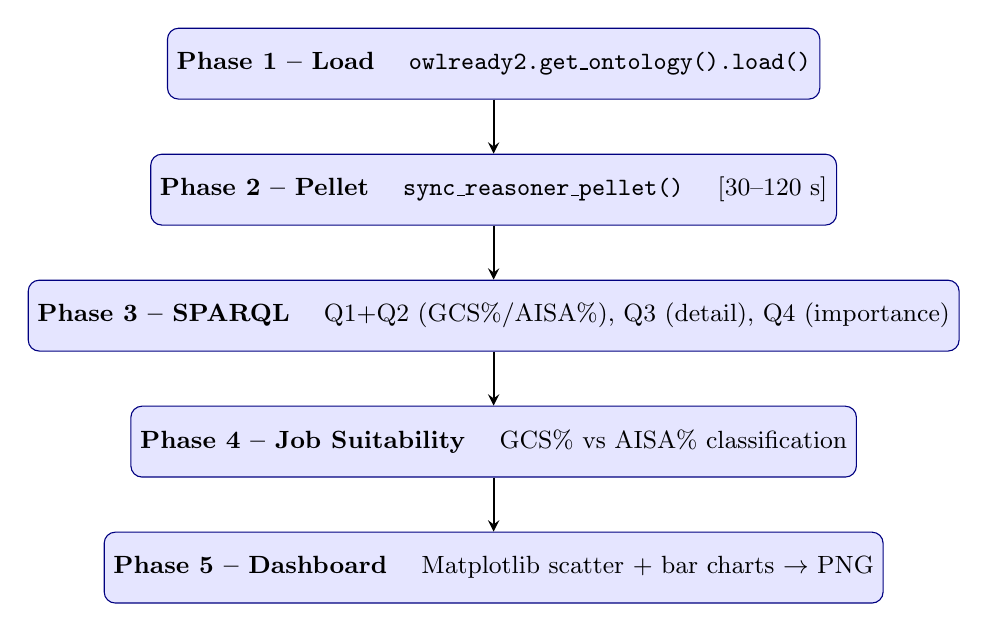
\begin{tikzpicture}[node distance=1.6cm, every node/.style={font=\small}]
  \tikzstyle{phase} = [rectangle, rounded corners, minimum width=8cm, minimum height=0.9cm,
                        text centered, draw=blue!50!black, fill=blue!10]
  \tikzstyle{arrow} = [thick,->,>=stealth]
  \node (p1) [phase] {\textbf{Phase 1 -- Load} \quad \texttt{owlready2.get\_ontology().load()}};
  \node (p2) [phase, below of=p1] {\textbf{Phase 2 -- Pellet} \quad \texttt{sync\_reasoner\_pellet()} \quad [30--120 s]};
  \node (p3) [phase, below of=p2] {\textbf{Phase 3 -- SPARQL} \quad Q1+Q2 (GCS\%/AISA\%), Q3 (detail), Q4 (importance)};
  \node (p4) [phase, below of=p3] {\textbf{Phase 4 -- Job Suitability} \quad GCS\% vs AISA\% classification};
  \node (p5) [phase, below of=p4] {\textbf{Phase 5 -- Dashboard} \quad Matplotlib scatter + bar charts $\rightarrow$ PNG};
  \draw [arrow] (p1) -- (p2);
  \draw [arrow] (p2) -- (p3);
  \draw [arrow] (p3) -- (p4);
  \draw [arrow] (p4) -- (p5);
\end{tikzpicture}
\end{center}

\subsection{Phase 3 -- Key SPARQL Query (Q1+Q2)}

\begin{lstlisting}[language=SPARQL]
SELECT ?person ?job ?skab ?score ?bfq ?ap1q WHERE {
    ?person  <isEvaluatedForJob>   ?job .
    ?person  <isSelected>          ?selected .
    FILTER(?selected = true)
    ?job     <requires>            ?jde .
    ?jde     <concerns>            ?skab .
    ?jde     <hasScore>            ?score .
    ?skab    <isTranslatedWithICFCode>  ?icf .
    ?person  <isInHealthCondition>      ?hc .
    ?hc      <isDescribedBy>            ?des .
    ?des     <involvesICFCode>          ?icf .
    OPTIONAL { ?des <BFqual>  ?bfq  }
    OPTIONAL { ?des <AP1qual> ?ap1q }
}
\end{lstlisting}

This joins the job-side (score) with the person-side (qualifier) via the shared ICF code.

\subsection{Phase 4 -- GCS\% and AISA\% Computation}

For each (Person, Job) pair and all $N$ associated SkAb:

\begin{align}
  \text{anchor}_i &= \begin{cases} 3 & \text{score} \geq 75 \\ 2 & \text{score} \in [50, 74] \\ 1 & \text{score} \in [26, 49] \\ 0 & \text{score} \leq 25 \end{cases} \\[6pt]
  \text{qualifier}_i &= \max(\texttt{BFqual}_i,\; \texttt{AP1qual}_i) \\[6pt]
  \text{CS}_i &= \text{qualifier}_i \times \text{anchor}_i \quad \in [0, 12] \\[6pt]
  \text{GCS\%} &= \frac{\sum_{i=1}^{N} \left(\text{CS}_i / 12\right)}{N} \times 100 \\[6pt]
  \text{AISA\%} &= \frac{|\{i : \text{CS}_i > 0\}|}{N} \times 100
\end{align}

\subsection{Phase 4 -- Job Suitability Thresholds}

Based on Figure~4 of the paper:

\begin{equation}
  \text{Suitability} = \begin{cases}
    \text{NOT SUITABLE} & \text{GCS\%} > -0.5 \times \text{AISA\%} + 21.0 \\
    \text{WITH PRECAUTIONS} & -0.5 \times \text{AISA\%} + 15.5 \leq \text{GCS\%} \leq -0.5 \times \text{AISA\%} + 21.0 \\
    \text{SUITABLE} & \text{GCS\%} < -0.5 \times \text{AISA\%} + 15.5
  \end{cases}
\end{equation}

\subsection{Criticality Labels}

\begin{longtable}{@{}ll@{}}
\toprule
\textbf{CS Value} & \textbf{Label} \\
\midrule
\endhead
0 & not critical \\
1--2 & SLIGHTLY CRITICAL \\
3--4 & MODERATELY CRITICAL \\
5--6 & RELEVANTLY CRITICAL \\
7--9 & EXTREMELY CRITICAL \\
\bottomrule
\end{longtable}

%% ─────────────────────────────────────────────────────────────
\\clearpage
\section{Known Issues and Notes}

\begin{tcolorbox}[colback=noteblue!40, colframe=blue!50!black, title=Note: ICF Inheritance Cycles]
The ICF class hierarchy contains cycles (a known limitation of the full ICF ontology). Pellet handles these with \texttt{TypeError: inheritance cycle} exceptions that are silently caught by a monkey-patch in \texttt{run\_pellet()}. This does not affect the reasoning output.
\end{tcolorbox}

\vspace{0.5em}

\begin{tcolorbox}[colback=warnred!40, colframe=red!60!black, title=Warning: hasSpecificCriticality Is Not Job-Specific]
Pellet writes a single \texttt{hasSpecificCriticality} triple per SkAb individual, without binding it to a specific job. As a result, CS values from this property are identical across different jobs for the same SkAb. The pipeline re-computes CS from \texttt{hasScore} (job-specific) and ICF qualifier directly to avoid this. The \texttt{hasSpecificCriticality} path remains as a fallback.
\end{tcolorbox}

\vspace{0.5em}

\begin{tcolorbox}[colback=importantbg!60, colframe=green!50!black, title=Important: isSelected Flag Is Mandatory]
The Q1+Q2 SPARQL query and the R1--R8 SWRL rules both filter on \texttt{isSelected = true}. If no \texttt{Person} individual has this flag set, no criticality triples are inferred and the pipeline falls back to the \texttt{hasSpecificCriticality} path, which may return job-identical results.
\end{tcolorbox}

%% ─────────────────────────────────────────────────────────────
\\clearpage
\section{Files and Dependencies}

\begin{longtable}{@{}ll@{}}
\toprule
\textbf{File} & \textbf{Role} \\
\midrule
\endhead
\texttt{Ontology/Rientra3.rdf} & Main ontology (OWL/RDF-XML) \\
\texttt{Program/ontology\_reasoner.py} & Reasoning pipeline (owlready2 + Pellet) \\
\texttt{Pattern Match/.../rdb2rdf\_step2.py} & Job matching pipeline (DB $\to$ ontology, NLP strategies) \\
\bottomrule
\end{longtable}

\noindent\textbf{Runtime requirements:}
\begin{lstlisting}
pip install owlready2 matplotlib rich
Java 11+ must be in PATH  (Pellet is invoked as a Java subprocess)
\end{lstlisting}

\end{document}

